\documentclass{beamer}
\usepackage{german}
\usepackage{lmodern}
\usepackage{tikz}
%

%
	
\begin{document}
\begin{frame}[t,shrink=65]

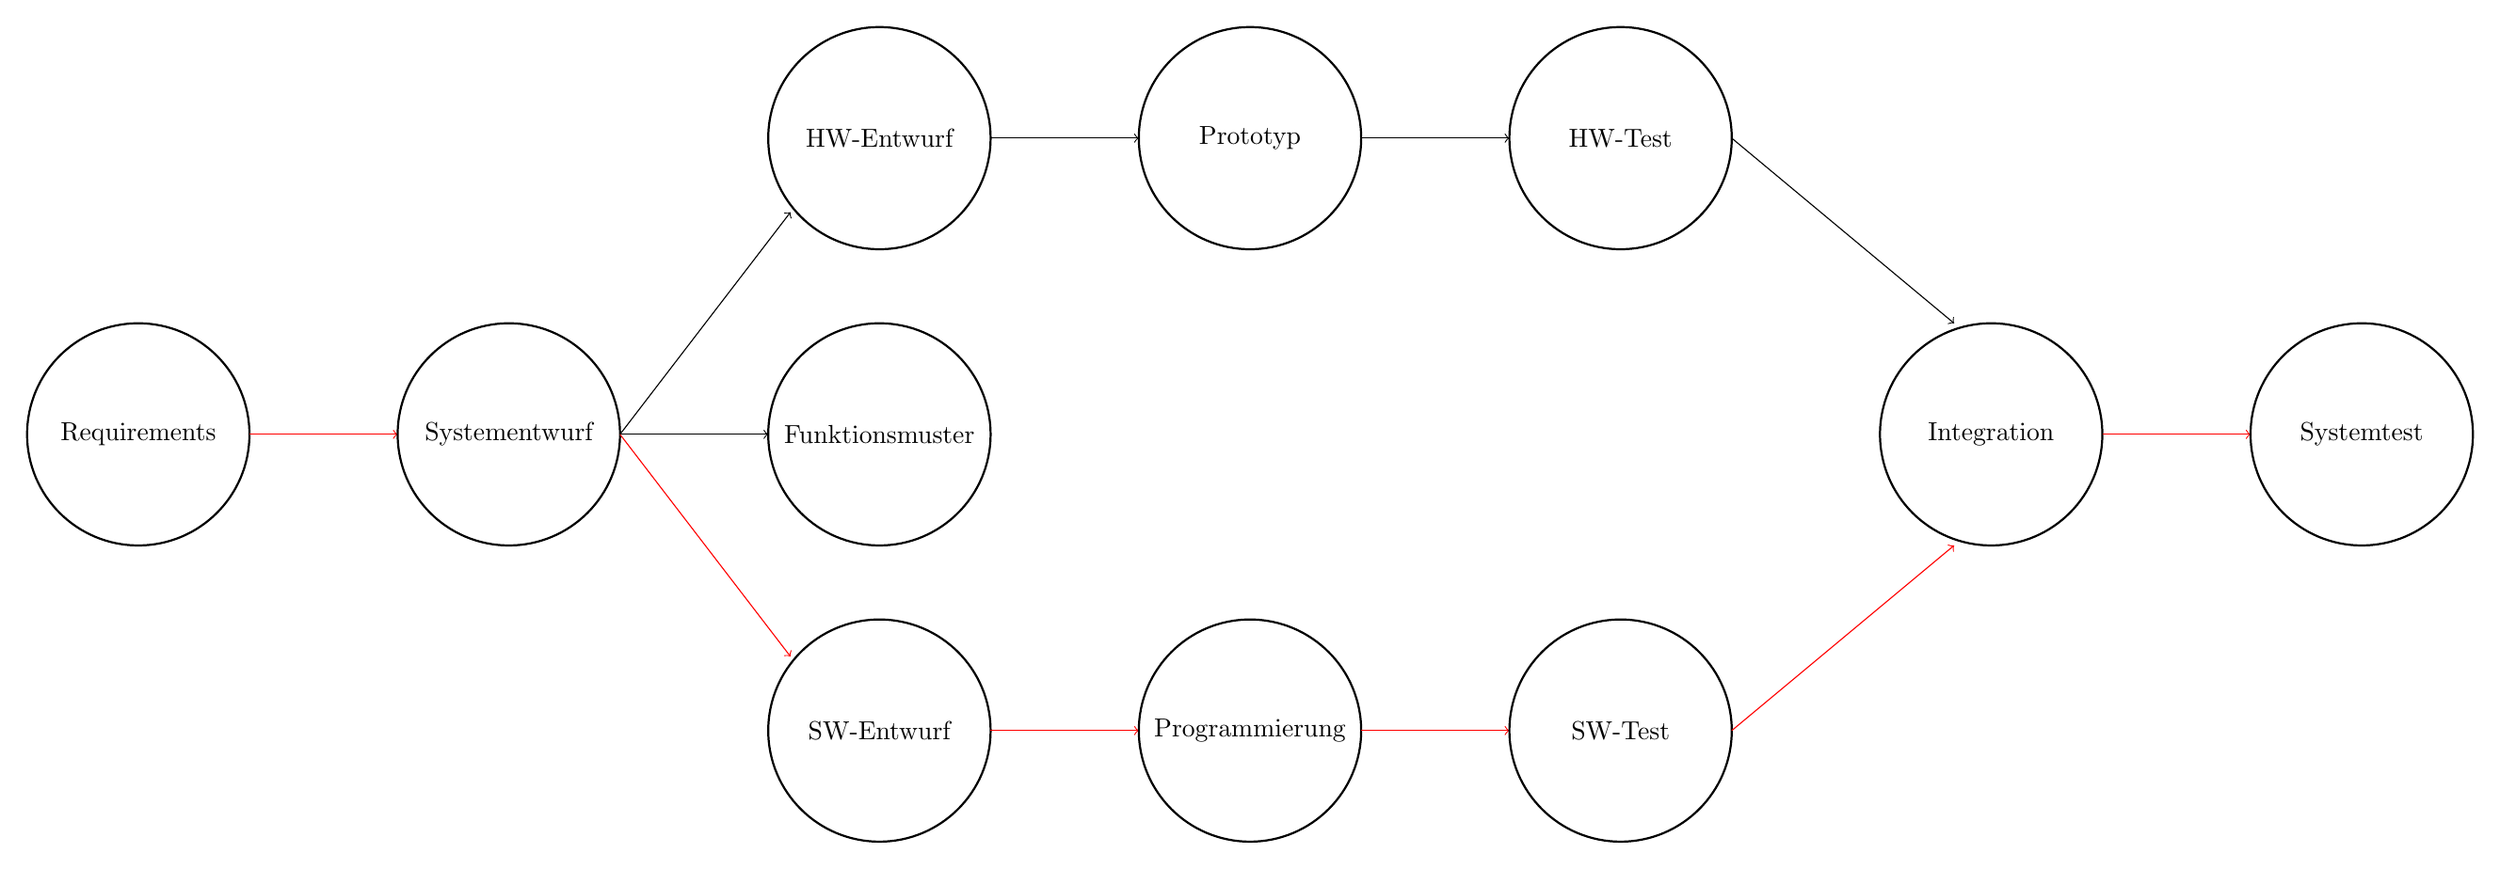
\begin{tikzpicture}
\draw[black, thick](0,0) circle(1.5) node {Requirements};
%\draw[thick] (-1,-1) -- (1,-1);
\draw[->, red] (1.5,0) -- (3.5,0);
\draw[black, thick](5.0,0) circle(1.5) node {Systementwurf};
\draw[->] (6.5,0) -- (8.8,3);
\draw[black, thick](10.0,4) circle(1.5) node {HW-Entwurf};
\draw[->] (6.5,0) -- (8.5,0);
\draw[black, thick](10.0,0) circle(1.5) node {Funktionsmuster};
\draw[->, red] (6.5,0) -- (8.8,-3);
\draw[black, thick](10,-4) circle(1.5) node {SW-Entwurf};
\draw[->] (11.5,4) -- (13.5,4);
\draw[black, thick](15,4) circle(1.5) node {Prototyp};
\draw[->,red] (11.5,-4) -- (13.5,-4);
\draw[black, thick](15,-4) circle(1.5) node {Programmierung};
\draw[->] (16.5,4) -- (18.5,4);
\draw[black, thick](20,4) circle(1.5) node {HW-Test};
\draw[->,red] (16.5,-4) -- (18.5,-4);
\draw[black, thick](20,-4) circle(1.5) node {SW-Test};
\draw[->,red] (21.5,-4) -- (24.5,-1.5);
\draw[black, thick](25,0) circle(1.5) node {Integration};
\draw[->] (21.5,4) -- (24.5,1.5);
\draw[->,red] (26.5,0) -- (28.5,0);
\draw[black, thick](30,0) circle(1.5) node {Systemtest};

\end{tikzpicture}

\mode<presentation>
\definecolor{hdaRot}{cmyk}{0,1,1,0.18}     % -5005
\definecolor{hdaBlauMed}{cmyk}{0.71,0.25,0,0}     % -1169
\definecolor{hdaGruenMed}{cmyk}{0.5,0.13,1,0.06}    % -2048

{\Large
	\par\vspace{2cm}\noindent  
	
    \begin{tabular}{l|lcccl}
      \hline
    Nr & Tätigkeit & Vorgänger & T$_{o}$ & T$_{w}$ & T$_{p}$ \\
     1  & Requirements & - & 1 & 2 & 3  \\
     2  & Studie & - & 1 & 1 & 2  \\
     3  & Sytsementwurf & 1 & 3 & 4  & 5  \\
     4  & 3 & 2 & -  \\
     5  & HW-Entwurf& 3 & 2 & 3 & 4 \\
     6  & Funktionsmuster  & 3 & 1.5  & 2 & 2.5 \\
     7  & SW-Entwurf  & 3 & 2.5  & 3 & 4 \\
     8  & Programmierung & 7 & 5 & 6 & 7.5 \\
     9  & 8  & 6 & -  \\
    10  & SW-Test & 8 &  4 & 5& 6 \\
    11  & Prototyp-Entwicklung & 5 & 4 & 5 & 6  \\
	12  & 11  & 6 & - & & \\
	13  & HW-Test  & 11 & 3 & 4 & 5 \\
	14  & Integration & 10;13 & 1 & 2 & 3 \\
	15  & Sytsem-Test & 14 & 2 & 3 & 4 \\
      \hline
        & \textbf{Gesamtaufwand} & \textbf{40}  \\
    \end{tabular}
}

\par\vspace{1cm}\noindent 
\begin{itemize}
{\huge
	 \item<only@+> {Dein Netzplan beginnt immer bei einem t$_{F}$ von 0.}
	 
	  \item<only@+> {Suche alle Vorgänge ohne Vorgänger (siehe Liste). Alle diese Pfeile gehen von unserem ersten Knoten aus. Schreibe die Tätigkeiten (in Kurzform), sowie Aufwand/Dauer auf den Pfeil.}
	  
	\item \alert<+> {}
}
\end{itemize}
	
\end{frame}

\end{document} 